\documentclass[8pt]{beamer}

\usepackage[utf8]{inputenc}
\usepackage{default}
\usepackage{hyperref}
\usepackage{textpos}
\usetheme{Copenhagen}

\title{Deep Learning}
\subtitle{Data encoding / representation}
\author{Tero Keski-Valkama}
\institute{
\includegraphics[height=1.4cm]{CybercomG_logo_Classic_RGB.png}}
\date{2016-09-22}

\addtobeamertemplate{frametitle}{}{%
\begin{textblock*}{100mm}(10.95cm,-0.8cm)

\includegraphics[height=0.8cm]{cybercom-blue.png}
\end{textblock*}}


\begin{document}

\frame{\titlepage}
 
\begin{frame}
\frametitle{A quick recap}
\begin{itemize}
 \item Deep learning refers to deep neural networks. 1990s networks were shallow, and hence relatively useless.
 \item Neural networks are just complex non-linear models with lots of parameters. They are formed by layers of neurons, successive operations
       with an a linear combination of inputs from the previous layer and a non-linear activation function.
 \item In general, you always need a training set, a test set and a validation set. Training set is used to tune parameters, test set is used to tune hyperparameters,
       and validation set is used to check that the model does not overfit the test set. Bootstrapping can be used to validate the data sectioning.
 \item Underfitting = high bias, overfitting = high variance
\end{itemize}

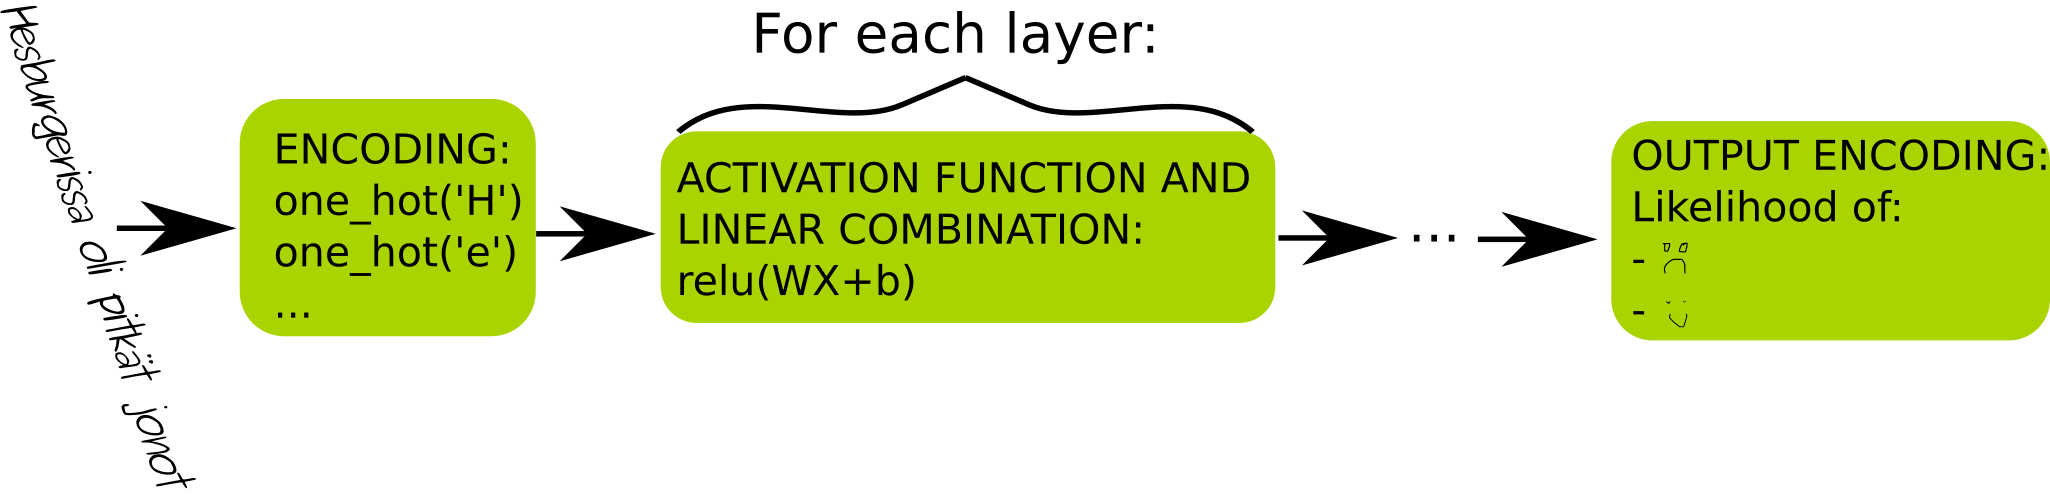
\includegraphics[width=0.9\textwidth]{./sentiment_analysis.png}

\end{frame}

\begin{frame}
\frametitle{Training Neural Networks}
\begin{itemize}
 \item In supervised training, the neural networks requires input and target output. The system finds a layered non-linear function from input to output.
 \item In unsupervised training, the network is only given input, and it learns a structure that captures the input statististical distributions and correlations.
 \item Unsupervised training uses energy-based methods which are better able to capture deep associations than a simple backpropagation, hence it is used for pre-training.
 \item A good platform to use for neural network experimentation is Google's TensorFlow, based on Python.
 \item Data representation is critical in neural networks, in the input representation, in the output representation (and by extension in defining the loss function), and
       also in the internal neuron representation.
 \item Training a neural network leads to neural layers forming a mapping from input data vector space through feature filters to higher level non-linear feature spaces and
       ultimately to semantic spaces.
\end{itemize}
\end{frame}

\begin{frame}
\frametitle{Tips \& Tricks}
 \begin{block}{Data Representation}
  \begin{itemize}
   \item Input representation
   \begin{itemize}
    \item Feature Engineering \& Dimensionality Reduction
    \item Trivial Representation \& Normalization
    \item Missing values
    \item Encoding time
    \item Local conditioning
   \end{itemize}
   \item Output representation
   \begin{itemize}
    \item Boolean values, Continuous values
    \item One-hot encoding for encoding exclusive choice
    \item Mixture distributions
   \end{itemize}
   \item Internal representation
   \begin{itemize}
    \item Feature spaces
   \end{itemize}
   \item Bonus: Residual and skip connections
  \end{itemize}
 \end{block}
\end{frame}

\begin{frame}
\frametitle{Input Representation / Feature Engineering \& Dimensionality Reduction}
 \begin{itemize}
  \item Dimensionality reduction is needed for cases where the signal is very high-dimensional (and possibly also high-bandwidth) and can be compressed
        without losing any meaningful information. That means removing correlating variables and variables with inconsequential variance. Note that low variance might also
        mean you need to normalize, so ``inconsequential'' does not mean exactly the same as ``low''.
  \item In the history, feature engineering was a pretty much the only way to make neural networks to do anything meaningful. Technically it means using higher brain functions
        to invent a coding for the signal that compresses the information heavily, leaving in only the features that are deemed central for the task at hand.
  \footnote{\href{http://machinelearningmastery.com/discover-feature-engineering-how-to-\\engineer-features-and-how-to-get-good-at-it/}
                 {http://machinelearningmastery.com/discover-feature-engineering-how-to-engineer-features-and-how-to-get-good-at-it/}}
  \item If you create a model that uses a reduced signal, then your model will be simpler and potentially more efficient.
 \end{itemize} 
\end{frame}

\begin{frame}
\frametitle{Input Representation / Feature Engineering \& Dimensionality Reduction}
 \begin{itemize}
  \item Feature selection is an art which requires understanding the application domain as well as understanding machine learning.
  \item Commonly used methods for dimensionality reduction is Principal Component Analysis, where you find the most significant eigenvector basis with few components for the data
        so that the loss in projecting the signal to that subspace is small.
  \footnote{\href{http://www.scholarpedia.org/article/Eigenfaces}
                 {http://www.scholarpedia.org/article/Eigenfaces}}
  \item Nowadays as computers are more efficient, feature engineering is not anymore in the central role it used to be in the past. However, it is good to understand that there
        is no such thing as ``raw encoding'', and all data must be represented and quantitized in some way, both in computer memories and in brains.
 \end{itemize} 
\end{frame}

\begin{frame}
\frametitle{Input Representation / Trivial Representation \& Normalization}
 \begin{itemize}
  \item If a neural network represents a function $ f(\mathbf{x}) = \mathbf{y} $, then input is a multidimensional vector $ \mathbf{x} $.
  \item The data is represented in a categorical fashion or as continuous values.
  \item 0/1 flag-like attributes are typically encoded simply as number components on the vector.
  \item Categories, such as words or letters are encoded as one-hot
        vectors where all the other components are marked as 0, but the component for the category as 1. Words as one-hot vectors tend to create really large vectors,
        unknown words cannot be represented, and typographically similar words are not close to each other.
  \item Continuous values are discretized into sequences. If a value is a continuous value between low and high limits, then a simple normalization between $ (0, 1) $
        is often in order.
  \item If a value does not have limits, tanh or sigmoid normalization might be used to clamp the value between $ (0, 1) $ or $(-1, 1) $.
  \item It is important to normalize the inputs so that they all have similar ranges. Otherwise the training concentrates on the large values only, disregarding the small ones.
        Also, the meaning of the signal should be somehow evident. If the signal is meaningfully continuous and the meaning comes from passing thresholds, then a continuous
        encoding is in order. But for example for waveforms and sounds it makes sense to use one-hot encoding.
 \end{itemize}
\end{frame}

\begin{frame}
\frametitle{Input Representation / Encoding Time}
 \begin{itemize}
  \item Fixed-rate sequences are easy for encoding. However, there are lots of data sources that are not fixed-rate.
  \item Delays and intervals are often important. Encoding delay as a single number works only if it is normalized between 0 and 1. However, this means that
        differences between short delays are much more significant than differences between long delays.
  \item Consider using ``tick'' events in variable-rate sequences. An LSTM network can more easily count ticks than associate to ad-hoc normalized delay components.
        (citation needed, ``trust but verify'')
  \item I have used such tick events in encoding Flexible Assembly System logs, and they work better than encoding delay as a scalar component.
 \end{itemize}
\end{frame}

\begin{frame}
\frametitle{Input Representation / Local conditioning}
 \begin{itemize}
  \item How to create networks that associate together low rate text with high rate audio signal?
  \item These are needed for voice synthesis and speech recognition systems.
  \item To condition the neural network with another signal requires the signals to be of the same rate. Consider for example lyrics and sound.
  \item Transposed convolution is often used to learn an upsampling for the lower rate signal. ``Deconv'' networks can learn even non-linear upsamplings.
        \footnote{\href{https://arxiv.org/abs/1603.07285}
                       {A guide to convolution arithmetic for deep learning}}
  \item Transposed convolution or fractional stride convolution is a kind of convolution that outputs larger signals than they are fed.
  \item These networks were originally called deconvolutional neural networks, but that is a misnomer, as deconvolution means an inverse operation to convolution,
        and this is not what transposed convolutions are.
  \item As the upsampling is learned, the network associates the lower rate signal to the higher rate signal matching the rates together.
        \footnote{\href{https://arxiv.org/abs/1606.05328v2}
                       { Conditional Image Generation with PixelCNN Decoders}}
  \item A soft, learned window can also be used to match the input window progress for separate sequences.
        \footnote{\href{http://arxiv.org/abs/1308.0850v5}
                       { Generating Sequences With Recurrent Neural Networks}}
 \end{itemize}
\end{frame}

\begin{frame}
\frametitle{Output Representation / Categorical and Class Outputs}
 \begin{itemize}
  \item Categorical outputs refer to a situation where the output can take one out of a limited set of values. These are used for example in classification tasks where
        the input signal is classified to represent one of predetermined classes. For example ``cat'' vs. ``dog'', or ``walking'' vs. ``driving''.
  \item For categorical outputs, one-hot softmax encoding is typically used. In generation, the outputs represent probabilities for picking a specific category.
  \item Softmax normalizes the sum of the output values to be one, and scales all values to be positive, i.e. forms a proper probability distribution.
  \item The loss is calculated using cross entropy. In Tensorflow, you skip the softmax layer in the loss function and use the unnormalized outputs (interpreted as log-probabilities)
        directly with the tf.nn.softmax\_cross\_entropy\_with\_logits function.
  \item Sometimes the outputs are not mutually exclusive. For example, a photo might contain both a cat and a person. In these cases you normalize each output
        between 0 and 1 using a sigmoid function. In Tensorflow, you would use tf.nn.sigmoid\_cross\_entropy\_with\_logits function to calculate the loss from raw, unscaled outputs.
 \end{itemize}
\end{frame}

\begin{frame}
\frametitle{Output Representation / Mixture Density Outputs}
 \begin{itemize}
  \item For continuous values, it makes sense to use mixture density distributions, that is, using a weighted mixture of several distributions (e.g. 3 x normal distributions) with
        parameters (for normal distribution: means and variances) estimated by the network.
  \item The relative weights are softmaxed to represent a discrete probability distribution, much like categorical outputs above.
  \item The distribution parameters are normalized to an appropriate range if necessary, for example variance of the normal distribution
        is typically transformed through exp() function to
        limit it to be always non-negative. This also has a rationale from statistical likelihoods.
  \item Generating values from mixture density distributions is done by first picking the distribution index from the set of distributions using the relative weight probabilities.
  \item Then a value is picked from the selected distribution using sampling from that kind of distribution with those parameters.
  \item Mixture density distributions work especially well for continuous physical signals where the system has several different ``decisions''
        to make from moment to moment. This corresponds to degrees of freedom in some sense.
  \item It is not always clear how many distributions you should use. Analogous to K-means clustering.
 \end{itemize}
\end{frame}

\begin{frame}
\frametitle{Output Representation / Audio}
 \begin{itemize}
  \item In audio signals, it has been noted that instead of using mixture density distributions it is better to use one-hot softmax classes for different
        signal values at a certain time.
  \item This corresponds to a discrete distribution, and it works better because it is not clear for audio signals how many mixtures one should use.
  \item To keep the output tractable, the signal levels are squashed from full 16 bit to for example 255 different values using $\mu$-law encoding.
        \footnote{\href{https://deepmind.com/blog/wavenet-generative-model-raw-audio/}
                       {WaveNet: A Generative Model for Raw Audio}}
 \end{itemize}
\end{frame}

\begin{frame}
\frametitle{Output Representation / Missing Values}
 \begin{itemize}
  \item Sometimes target output data is missing values. For example, you have an image segmentation application that labels regions in the image as trees or cats.
        Your training output data has some regions marked as belonging to a specific label in rough brush strokes, or ``scribbles''. Most of the area in the image is not labelled.
  \footnote{\href{http://arxiv.org/pdf/1604.05144v1.pdf}
                 {ScribbleSup: Scribble-Supervised Convolutional Networks for Semantic Segmentation}}
  \item Related terms: Weakly supervised learning, partial labels, superpixel segmentation.
  \footnote{\href{http://www.cv-foundation.org/openaccess/content\_cvpr\_2015/papers/Xu\_Learning\_to\_Segment\_2015\_CVPR\_paper.pdf}
       {Constrained Convolutional Neural Networks for Weakly Supervised Segmentation}}
  \item Superpixel segmentation means clustering the pixels in the 5-dimensional color+spatial space.
  \item Unmarked pixels are marked by propagating supervised values on the superpixel,
        but also propagating pixelwise predictions of the neural network backwards.
  \item Handling of missing values in general depends on the application.
        
 \end{itemize} 
\end{frame}

\begin{frame}
\frametitle{Internal Representation / Feature Space Representation}
 \begin{itemize}
  \item Interpolating representations in feature and semantic spaces generate cognitive morphings.
  \item Interpolation in explicit feature space and transposed convolution:
        \href{https://www.youtube.com/watch?v=QCSW4isBDL0}{Learning to Generate Chairs with Convolutional Neural Networks}
  \item Interpolation in implicit feature space:
        \href{https://arxiv.org/abs/1606.05328}{Conditional Image Generation with PixelCNN Decoders}
  \item Internal representation for text allows arithmetic in the meaning space.
  \item \href{http://deeplearning4j.org/word2vec.html}{Word2Vec}: Learning 100-1000 dimensional embeddings for words based on their context with a 2-layer neural network
        predicting the current word based on context. For internal representation, interesting applications follow: Brother - Man + Woman = Sister.
  \item Understanding internal encoding and representation is crucial for interrogating neural networks. See also: \href{http://arxiv.org/pdf/1410.3916v11.pdf}{MemNN}
        \footnote{\href{http://www.pamitc.org/cvpr15/files/lecun-20150610-cvpr-keynote.pdf}{Yann Le Cunn: What's Wrong With Deep Learning?}}
 \end{itemize}
\end{frame}

\begin{frame}
\frametitle{Bonus: Residual and Skip Connections}
 \begin{itemize}
  \item Training deep neural networks requires all sorts of tricks, some of which were handled in the previous lecture.
  \item Current state of the art convolutional networks are in fact trained with backpropagation only, but require additional tricks.
  \item In deep learning, naive backpropagation struggles in pushing back the loss through the layers, and rather uses the biases to make bets, driving the weights to zero.
        It causes the information to stop flowing from input to output.
  \item Residual connections are connections that skip one layer in an additive fashion.
        The input of a unit is simply added to the output also. Sometimes a rectifier activation is added after the summation.
        This propagates the loss gradients backwards better during training, and information forwards better during generation.
        \footnote{\href{https://arxiv.org/abs/1512.03385}{Deep Residual Learning for Image Recognition}}
 \end{itemize}
\end{frame}

\begin{frame}
\frametitle{What did we learn?}
 \begin{itemize}
  \item To make neural networks learn effectively, the data must be represented in a suitable fashion.
  \item Creating more complex neural network architectures for the purposes or combining different and variable rate signals,
        or interrogating neural networks, one needs a good intuition about the feature spaces in the internal representation.
  \item Interpolating internal representation or performing algebraic operations on them is useful in a number of applications.
        The distance between two internal representation vectors typically tell us about semantic distances between the inputs.
  \item Output representations are intricately tied to loss functions.
  \item Also, thanks to Jussi Lyytinen, who helped with the data science and statistics perspective.
 \end{itemize}
\end{frame}

\end{document}

